%\documentclass[11pt,a4paper,uplatex,dvipdfmx]{ujarticle} 		% for uplatex
\documentclass[11pt,a4j,dvipdfmx]{jarticle} 					% for platex
%=======================================
% form00_header.tex
%	General header for kakenhiLaTeX,  Moved over from form00_2010_header.tex.
%	2009-09-06 Taku Yamanaka (Osaka Univ.)
%==== General Version History ======================================
% 2006-05-30 Taku Yamanaka (Physics Dept., Osaka Univ.)
% 2006-06-02 V1.0
% 2006-06-14 V1.1 Use automatic calculation for cost tables.
% 2006-06-18 V1.2 Split user's contents and the format.
% 2006-06-20 V1.3 Reorganized user and format files
% 2006-06-25 V1.4 Readjusted all the table column widths with p{...}.
%				With \KLTabR and \KLTabRNum, now the items can be right-justified
%				in the cell defined by p{...}.
% 2006-06-26 V1.5 Use \newlength and \setlength, instead of \newcommand, to define positions.
% 2006-08-19 V1.6 Remade it for 2007 JFY version.
% 2006-09-05 V1.7 Added font declarations suggested by Hoshino@Meisei Univ.
% 2006-09-06 V1.8 Introduced usePDFform flag to switch the form file format.
% 2006-09-09 V1.9 Changed p.7, to allow different heights between years. (Thanks to Ytow.)
% 2006-09-11 V2.0 Added an option to show budget summary.
% 2006-09-13 V2.1 Added an option to show the group.
% 2006-09-14 V2.1.1 Cleaned up Kenkyush Chosho.
% 2006-09-21 V2.2 Generated under a new automatic development system.

% 2007-03-24 V3.0 Switched to a method using "picture" environment.

% 2007-08-14 V3.1 Switched to kakenhi3.sty.
% 2007-09-17 V3.2 Added \KLMaxYearCount
% 2008-03-08 V3.3 Remade it for 2009 JFY version\
% 2008-09-08 V3.4 Added \KLXf ... \KLXh.
% 2011-10-20 V5.0 Use kakenhi5.sty, to utilize array package in tabular environment.
% 2012-08-14 v5.1 Moved preamble and kakenhi5 into the current directory, instead of the parent directory.
% 2012-11-10 v6.0 Switched to kakenhi6.sty.
% 2015-08-26 v6.1 Added KLFirstPageIsLongPage flag.
% 2017-05-27 v7.0 Simplified for the new format.
%=======================================
% Dummy section and subsection commands.
% With these, some editors (such as TeXShop, etc.) can jump to the (sub)sections.
\newcommand{\dummy}{dummy}% 
\renewcommand{\section}[1]{\renewcommand{\dummy}{#1}}

\usepackage{calc}
\usepackage{geometry}                % See geometry.pdf to learn the layout options. There are lots.
\usepackage[dvipdfmx]{graphicx}
\usepackage{color}
\usepackage{ifthen}
\usepackage{udline}
\usepackage{array}
\usepackage{longtable}
\usepackage{fancyhdr}
 % pieces
%==================================================
% kakenhi7.sty
%==================================================
% v1
% Minimum amount of macros for writing Kakenhi forms.
%
% 2005-10-24 Taku Yamanaka, Physics Dept. Osaka Univ.
%		taku@hep.sci.osaka-u.ac.jp
% 		Macros such as XYBC, etc. were imported from Kakenhi Macro at
% 		http://www.yukawa.kyoto-u.ac.jp/contents/researcher/kakenhi.html .
% 2006-06-04 Taku
%		Added macros to draw boxes if \DrawBox is in the source.
%		This is useful when designing the LaTeX forms.
% 2006-06-14 Taku
%		Added LaTeX macros to add costs 
%		(\KLResetGrandSum, \KLCostItem, \KLSum, \KLGrandSum).
%		Added a macro \Number to supply commas every 3 digits (imported from kkh.mac).
% 2006-06-25 Taku
%		Added \KLTabC, \KLTabR, \KLTabRNum to specify alignments in tables.
%		Please note that \phantom{...} is required for the column, 
%		or otherwise somehow p{...mm} is ignored.
% 2006-08-13 Taku
%		Added \KLItemNumUnitCost . This requires calc.sty.
% 2006-09-06 Taku
%		Added KLGrandTotalValue to add ALL the costs.
%		Also added \KLPrintGrandTotal to print the total on the console.
% 2006-09-09 Taku
%		Added macros to handle "efforts".
% 2006-09-10 Taku
%		Added \KLnewcounter to make series of counters.
%		Modified \KLResetGrandSum and \KLSum to add the sum for 
%		each category and year.
% 2006-09-11 Taku
%		Added \NumC to display LaTeX counter with commas.
% 2006-09-12 Taku
%		Added simple macros to make group table.
% 2006-09-23 Taku
%		Added the 'Fair License' notification.
% 2006-10-22 Taku
%		Initialize KLNumPeople to -1, so that the first header row will not be included in the count.
%====================================================
% v2
% 2007-03-24 Taku
%		Instead of using Kakenhi Macros to position items, 
%		switched to a new method using
%		"picture" environment.  The origin of the coordinate is set to 
%		the lower left corner of the paper.  The positions are given in "points", 
%		as can be read by gv. These methods were suggested by 
%		Tsutomu Sakurai at Saitama Univ..
% 2007-03-30 Taku
%		The sum of each category and year is made using 
%		macros \KLItemCost, etc., instead of \KLSum.  This is a step toward
%		automatically aligning category sums in the same year, in some forms.
% 2007-04-02 Taku
%		Added \KLBudgetMiniTabular, \KLMiniSum, etc. to handle
%		budget tables with multiple category columns.
% 2007-05-04 Taku
%		Added \multicolumnDottedLine .
%==================================================
% v3 
% 2007-08-14 Taku
%		Simplified page handling, by introducing \KLBeginSinglePage,
%		\KLPageRange, etc..
% 2007-09-01 Taku
%		Added a new command, \KLItemNumUnitCostLocation , 
%		and \KLAddCost to clean things up.
% 2007-09-06 Taku
%		Set \KLEven/OddLeft/RightEdge parameters in \KLWaterMark.
%		Without it, if \KLLeftEdge or \KLRightEdge is used inside watermark,
%		it generated a very obscure error message, which was hard to track down.
% 2007-09-09 Taku
%		Removed clearring \thiswatermark in \KLClearWaterMarks.
% 2007-09-12 Taku
%		Added \KLPriorityItemNumUnitCostTwo for Tokusui.
% 2007-09-14 Taku
%		Added \KLItemNumUnitCostTwo for tokutei_koubo.
% 2007-09-17 Taku
%		In \KLAddCost, costs are added only if it is within the defined year range.
% 2008-09-02 Taku
%		  Added \KLMonthPriorityItemNumUnitCostTwo for tokutei_keizoku.
% 2008-09-07 Taku
%		   Use \KLJFY to print year in budget tables.
% 2008-10-21 Taku
%			Added KLItemNumUnitCostInParen for shorei.
% 2009-09-03 Taku
%			Added \dottedLine .
%==================================================
% v4
% 2009-09-06 Taku
%			Added macros for partial typesetting.
% 2009-09-12 Taku
%			Added macros for showing coordinates and edges.
% 2009-09-13 Taku
%			Added macros to show boxes and minipage frames and their corner coordinates.
% 2010-03-04 Taku
%			Moved macros for calculating lengths and positions from form07_header.tex to here.
% 2010-04-11 Taku
%			Added \KLItemCostOne for jisedai, and necessary flags to print budget sums before 
%			the detailed budget table.
%==================================================
% v5
% 2011-10-20 Taku
%			By using array package within tabular environment, the following macros were simplified:
%			\KLTabC, \KLTabR, \KLBudgetMiniTabular, 
%			New Macros:
%			\KLCC, \KLCR
% 2011-10-24 Taku
%			Removed using \KLTabR from most of the budget tables.
% 2011-10-26 Taku
%			Added KLMyBudget.
%			Modified KLYearItemNumUnitCostTwo to just put the JFY if the second item is blank.  (For Kiban S)
% 2012-03-10 Taku
%			Changed the tabcolsep for \KLMyBudget to 0pt.
% 2012-08-14 Taku
%			Moved xxx_forms_pdf and _eps directories to under mother.
% 2012-09-09	Taku
%			Added \KLbibitem(B) and \KLcite(B).
% 2012-09-16	Taku
%			Added \KLOtherApplication, \KLOtherApplicationReasons, and \KLOtherFundReasons
%			for tokusui (and maybe for others in the future).
%==================================================
% v6
% 2012-11-10	Taku
% 			Modified \KLOtherApplicationReasons and \KLOtherFundReasons to make the tables compact.
%			These were in hook3.tex for the 2013 version.
%			Added \KLOtherApplicationDiff for many shumokus.
%			Removed \KLbibitemB and \KLciteB.
%			Changed \KLbibitem to use a dedicated column for numbering.
% 2012-11-11	Taku
%			Added \KLItemSetCostLocationInfo and \KLItemCostInfo.
% 2013-09-19	Taku
%			Added \KLOtherPD and \KLOtherPDShort to enter JSPS PD for other funds.
% 2013-10-02	Taku
%			Changed \KLbibItem, not to use a dedicated column for numbering, 
%			because otherwise the label defined in \label{...} cannot be used in @currentlabel.
% 2014-09-22	Taku
%			Added \KLCL for filling narrow tabular cells in English.  
%			(Suggested by Frank Bennett.)
% 2014-11-08	Taku
%			Added an instruction in \KLCheckPageLimit.
% 2015-08-23	Taku
%			Added NumCk to show numbers divided by 1000 (truncated).
% 2015-08-24	Taku
%			Introduced \KLLongPage and \KLSimpleLongPage to offer floating environment in 
%			single-page-frames.
%=====================================================
% v7
%	Frames are gone!  Simplify kakenhiLaTeX to benefit from 
%	the new style.
% 2017-05-03	Taku
%			Added \KLAnotherFund .
% 2017-05-27	Taku
%			Made \KLBeginSubject and \KLEndSubject to handle new 
%			mother file style.
% 2017-08-17 Taku
%	Added \KLItemCostNoYear and \KLEndBudgetNoYear for kokusai_kyoudou.
% 2017-08-19	Taku
%			Updated \KLBeginSubject and \KLEndSubject to handle 
%			various headers.
% 2017-08-20	Taku
%			\KLBeginSubject calls \KLFirstPageStyle and \KLDefaultPageStyle
%			which should be defined for each shumoku (or JSPS/MEXT).
%			This is to pass the subject name etc. to the header.
% 2017-08-27	Taku
%			Set section number in \KLBeginSubject.
% 2017-08-29	Taku
%			Moved over KLShumokuFirstPageStyle and KLShumokuDefaultPageStyle.
%			Added jsps-abs-p1-header, jps-abs-subject-header, and 
%			jsps-abs-default-header as arguments to \KLShumoku***Header.
% 2017-09-02	Taku
%			Added \KLBeginSubjectWithHeaderCommands for more flexible header style.
% 2017-09-03	Taku
%			Added \vspace*{-4mm} after \includegraphics in \KLBeginSubject*.
% 2017-09-05	Taku
%			Removed now-the-old commands.
% 2020-01-02	Taku
%			Added more numbers to \KLJint for gakuhen_a.
% 2020-01-15	Taku
%			Changed the horizontal position (none --> -3mm) 
%			and the width of the top boxes for headers (\linewidth --> 1.02\linewidth)
%			to reproduce the original boxes.  
%			This became necessary because the margins were set correctly in form02_header.tex.
% 2021-01-29	Taku
%			Set section counter and reset subsection counter only if the section # is given for
%			\KLBeginSubject and \KLBeginSubjectWithHeaderCommands .
% 2022-01-26	Taku
%			Changed the scale for the top boxes from 1.03 to 1.01, 
%			and \hspace from -3mm to -2mm.  (DC)
%=====================================================

%=====================================================
% Macro to supply commas every 3 digits (up to 9 digits)
%	Imported from kkh.mac for Kakenhi Macro.
%=====================================================
%
\newif\ifNumWithCommas \NumWithCommastrue
\def\NumWithCommas{\NumWithCommastrue}
\def\NumWithoutCommas{\NumWithCommasfalse}
\newcount\Numa
\newcount\Numb
\def\Numempty{}%output blank if "-0" is given
\def\Number#1{\edef\Numpar{#1}\ifx\Numempty\Numpar\else%
\ifNumWithCommas\Numa=#1\relax
\ifnum\Numa>999999\divide\Numa by 1000000
\number\Numa,%
\multiply\Numa by -1000000\advance\Numa by #1\relax
\Numb=\Numa\divide\Numa by 1000
\ifnum\Numa<100 \ifnum\Numa<10 0\fi0\fi\number\Numa,%
\multiply\Numa by -1000\advance\Numa by \Numb
\ifnum\Numa<100 \ifnum\Numa<10 0\fi0\fi\number\Numa%
\else\ifnum\Numa>999\divide\Numa by 1000
\number\Numa,%
\multiply\Numa by -1000\advance\Numa by #1\relax
\ifnum\Numa<100 \ifnum\Numa<10 0\fi0\fi\number\Numa%
\else\number\Numa\fi\fi\else\number#1\fi\fi}

%======================================================
% Macro to display LaTeX counter with commas every 3 digits.
%======================================================
\newcommand{\NumC}[1]{\Number{\value{#1}}}

\newcounter{kyen}
\newcommand{\NumCk}[1]{%
	\setcounter{kyen}{\arabic{#1}/1000}
	\Number{\value{kyen}}
}

%======================================================
% Macros to align (right-justify, center) elements within a tabular cell
% whose width is defined by p{...}.
% 2006-06-25 Taku
% 	These are necessary, because the cell width should be given explicitly
% 	by p{...mm} to match the given table in a tabular environment.  
% 	One could allocate a width with \phantom{...},
% 	but it is a little tricky, since it depends on the font size.
%======================================================

%---------------------------------------------------------------------
% Center text within a tabular cell allocated by p{...}
%\newcommand{\KLTabC}[1]{\multicolumn{1}{c}{#1}}
\newcommand{\KLTabC}[1]{\centering\arraybackslash#1}
% This new method does not require a dummy table row to put them in correct columns.
%
% This should be used in tabular definition, as:
%	\begin{tabular}[t]{>{\KLCC}p{30pt}p{50pt}}
\newcommand{\KLCC}{\centering\arraybackslash}

%---------------------------------------------------------------------
% Right justify text within a tabular cell allocated  by p{...}
%\newcommand{\KLTabR}[1]{\multicolumn{1}{r@{\ }}{#1}}
\newcommand{\KLTabR}[1]{\raggedleft\arraybackslash#1}

% This should be used in tabular definition, as:
%	\begin{tabular}[t]{>{\KLCR}p{30pt}p{50pt}}
\newcommand{\KLCR}{\raggedleft\arraybackslash}%

%---------------------------------------------------------------------
% Right justify number (with comma every 3 digits) 
% within a tabular cell allocated by p{...}
\newcommand{\KLTabRNum}[1]{\KLTabR{\Number{#1}}}

%---------------------------------------------------------------------
% Left justify text within a tabular cell allocated by p{...}
% This should be used in tabular definition, as:
%	\begin{tabular}[t]{>{\KLCL}p{30pt}p{50pt}}
\newcommand{\KLCL}{\raggedright\arraybackslash}%

%=================================================
%  counter tools
%=================================================
\newcounter{KLtmp}

%------------------------------------------------------------------------------
% Makes a set of counters, with prefix #1, followed by 
% suffix ranging from 0 to #2 - 1.
% For example, \KLnewcounter{mine}{3} makes counters
% mine0, mine1, and mine2 .
%-------------------------------------------------------------------------------
\newcommand{\KLnewcounter}[2]{
	\setcounter{KLtmp}{0}
	
	\whiledo{\value{KLtmp} < #2}{
		\newcounter{#1\arabic{KLtmp}}
		\stepcounter{KLtmp}
	}
}

%------------------------------------------------------------------------------
% Dumps the contents of the counters.
%------------------------------------------------------------------------------
\newcommand{\KLdumpcounter}[2]{
	\setcounter{KLtmp}{0}
	
	\whiledo{\value{KLtmp} < #2}{
		#1\arabic{KLtmp} : \arabic{#1\arabic{KLtmp}}\\
		\stepcounter{KLtmp}
	}
}

%=======================================================
% LaTeX macros to add costs.
%	2006-06-14 Taku Yamanaka
%=======================================================
\newcounter{KLCost}				% to calculate cost = #units x unit cost
\newcounter{KLGrandTotalValue}		% for the grand total of all the categories in all years
\setcounter{KLGrandTotalValue}{0}

\newcommand{\KLCostCategory}{KLequipments}
\newcounter{KLYearCount}
\newcounter{KLPrintYear}

% Make counters for annual sums for each category-----------------------
\newcommand{\KLMaxYear}{8}
\KLnewcounter{KLequipments}{\KLMaxYear}
\KLnewcounter{KLexpendables}{\KLMaxYear}
\KLnewcounter{KLdomestic}{\KLMaxYear}
\KLnewcounter{KLforeign}{\KLMaxYear}
\KLnewcounter{KLtravel}{\KLMaxYear}
\KLnewcounter{KLgratitude}{\KLMaxYear}
\KLnewcounter{KLmisc}{\KLMaxYear}
\KLnewcounter{KLAnnualSum}{\KLMaxYear}

%------------------------------------------------
% Add up the given cost to category-year sum, category sum, year-sum, and total.
% 2007-09-01 Taku
% 2007-09-17 Taku: Add costs only if it is within the defined year range.
%------------------------------------------------
\newcommand{\KLAddCost}[1]{%
	\ifthenelse{\value{KLYearCount} > \value{KLMaxYearCount}}{%
		%pass
	}{%
		\addtocounter{\KLCostCategory0}{#1}%
		\addtocounter{\KLCostCategory\arabic{KLYearCount}}{#1}%
		\addtocounter{KLAnnualSum\arabic{KLYearCount}}{#1}%
		\addtocounter{KLAnnualSum0}{#1}%
		\ifthenelse{\equal{\KLCostCategory}{KLdomestic}}{%
			\addtocounter{KLtravel0}{#1}%
			\addtocounter{KLtravel\arabic{KLYearCount}}{#1}%
		}{}%
		\ifthenelse{\equal{\KLCostCategory}{KLforeign}}{%
			\addtocounter{KLtravel0}{#1}%
			\addtocounter{KLtravel\arabic{KLYearCount}}{#1}%
		}{}%
	}%
}


\newcommand{\KLClearWaterMarks}{%
	%--empty watermarks
	\watermark{}
%	\thiswatermark{}
	\rightwatermark{}
	\leftwatermark{}
}

\newcommand{\KLInput}[1]{%	The macros defined inside the file are only valid within the file.
	\begingroup
	\input{#1}
	\endgroup
}

%================================
% For 2017 new style without frames
%================================
\newcommand{\KLShumokuFirstPageStyle}[5]{%
%	Defines the header for the first page.
%	Called from \KLBeginSubject.
%--------------------------------
%	#1: page style name
%	#2: 様式
%	#3: 研究種目名
%	#4: 項目名
%	#5: sectionNo
%--------------------------------
	\ifthenelse{\equal{#1}{jsps-p1-header}}{%
		\JSPSVeryFirstPageStyle{#1}{#2}{#3}{#4}{#5}
	}{%
		\ifthenelse{\equal{#1}{jsps-abs-p1-header}}{%
			\JSPSVeryFirstPageStyle{#1}{#2}{#3 概要}{#4}{#5}
		}{%
            		\ifthenelse{\equal{#1}{jsps-subject-header}}{%
            			\JSPSFirstSubjectPageStyle{#1}{#2}{#3}{#4}{#5}
            		}{%
				\ifthenelse{\equal{#1}{jsps-abs-subject-header}}{%
            				\JSPSFirstSubjectPageStyle{#1}{#2}{#3 概要}{#4}{#5}
				}{%
                    			\thispagestyle{#1}
				}
            		}
		}
	}
}

\newcommand{\KLShumokuDefaultPageStyle}[5]{%
%	Defines the default header.
%	Called from \KLBeginSubject.
%--------------------------------
%	#1: page style name
%	#2: 様式
%	#3: 研究種目名
%	#4: 項目名
%	#5: sectionNo
%--------------------------------
	\ifthenelse{\equal{#1}{jsps-default-header}}{%
		\JSPSDefaultPageStyle{#1}{#2}{#3}{#4}{#5}
	}{%
		\ifthenelse{\equal{#1}{jsps-abs-default-header}}{%
			\JSPSDefaultPageStyle{#1}{#2}{#3 概要}{#4}{#5}
		}{%
            		\pagestyle{#1}
		}
	}
}

\newcommand{\KLSubjectName}{}
\newcommand{\KLSubjectMaxPages}{}
\newcommand{\KLSubjectEndPage}{}
\newcounter{KLSubjectEndPage}
\setcounter{KLSubjectEndPage}{0}

\newcommand{\KLSubjectCheckNPages}{%
%	\arabic{page}, \arabic{KLSubjectEndPage}\\
	\ifthenelse{\value{page}>\value{KLSubjectEndPage}}{
		{\LARGE「\KLSubjectName」は \KLSubjectMaxPages\ ページ以内で書いてください。}
		\clearpage
	}{%
	}
}

\newcommand{\KLSubjectAdvancePages}{%
	\renewcommand{\KLSubjectEndPage}{\value{KLSubjectEndPage}}
	\ifthenelse{\value{page}<\KLSubjectEndPage}{%
		\phantom{x}\clearpage
	}{}
	% Advance page if necessary
	\ifthenelse{\value{page}<\KLSubjectEndPage}{%
		\phantom{x}\clearpage
	}{}
	% Advance page if necessary
	\ifthenelse{\value{page}<\KLSubjectEndPage}{%
		\phantom{x}\clearpage
	}{}
	% Advance page if necessary
	\ifthenelse{\value{page}<\KLSubjectEndPage}{%
		\phantom{x}\clearpage
	}{}
	% Advance page if necessary
	\ifthenelse{\value{page}<\KLSubjectEndPage}{%
		\phantom{x}\clearpage
	}{}
}	

\newcommand{\KLJInt}[1]{%
% Returns full-width numerical character.
	\ifthenelse{\equal{#1}{1}}{1}{%
	\ifthenelse{\equal{#1}{2}}{2}{%
	\ifthenelse{\equal{#1}{3}}{3}{%
	\ifthenelse{\equal{#1}{4}}{4}{%
	\ifthenelse{\equal{#1}{5}}{5}{%
	\ifthenelse{\equal{#1}{6}}{6}{%
	\ifthenelse{\equal{#1}{7}}{7}{%
	\ifthenelse{\equal{#1}{8}}{8}{%
	\ifthenelse{\equal{#1}{9}}{9}{%
	\ifthenelse{\equal{#1}{10}}{10}{%
	\ifthenelse{\equal{#1}{11}}{11}{%
	\ifthenelse{\equal{#1}{12}}{12}{%
	\ifthenelse{\equal{#1}{13}}{13}{%
	\ifthenelse{\equal{#1}{14}}{14}{%
	\ifthenelse{\equal{#1}{15}}{15}{%
	\ifthenelse{\equal{#1}{16}}{16}{%
	\ifthenelse{\equal{#1}{17}}{17}{%
	#1}}}}}}}}}}}}}}}}}%
}


\newcommand{\KLBeginSubject}[8]{%
%----------------------------------------------------
%	#1: subjectNo
%	#2: sectionNo
%	#3: sectionJ
%	#4: maxPages
%	#5: pageLengthStyle ('V' for variable, 'F' for fixed)
%	#6: pageCounter (set page counter to this value if the argument exists.
%	#7: subjectFirstPageHeader (header for the first page)
%	#8: defaultPageHeader
%----------------------------------------------------
	\ifthenelse{\equal{#2}{}}{%
	}{%
	    	\setcounter{section}{#2}
	    	\setcounter{subsection}{0}
	}
	\setcounter{subsubsection}{0}
	\renewcommand{\KLSubjectName}{#3}
	\renewcommand{\KLSubjectMaxPages}{#4}
	
	\ifthenelse{\equal{#6}{}}{%
	}{%
		\setcounter{page}{#6}
	}
	
	\setcounter{KLSubjectEndPage}{\value{page}}
	\addtocounter{KLSubjectEndPage}{#4}
	
	\ifthenelse{\equal{#7}{}}{%
		% pass
	}{%
		\KLShumokuFirstPageStyle{#7}{\様式}{\研究種目header}{#3}{#2}
	}
	
	\ifthenelse{\equal{#8}{}}{%
		% pass
	}{%
		\KLShumokuDefaultPageStyle{#8}{\様式}{\研究種目header}{#3}{#2}
	}
	
	\noindent
	\hspace{-2mm}
	\includegraphics[width=1.01\linewidth]{subject_headers/\KLYoshiki_#1.pdf}\\
	\vspace*{-4mm}
}

\newcommand{\KLNullHeader}[5]{}
% Dummy command for No header.
% This was introduced to avoid error caused in statement \ifthenelse{\equal{#8}{}} .

\newcommand{\KLBeginSubjectWithHeaderCommands}[8]{%
%----------------------------------------------------
%	#1: subjectNo
%	#2: sectionNo
%	#3: sectionJ
%	#4: maxPages
%	#5: pageLengthStyle ('V' for variable, 'F' for fixed)
%	#6: pageCounter (set page counter to this value if the argument exists.
%	#7: LaTeX command for subjectFirstPageHeader (header for the first page)
%	#8: LaTeX command for defaultPageHeader
%----------------------------------------------------
	\ifthenelse{\equal{#2}{}}{%
	}{%
		\setcounter{section}{#2}
		\setcounter{subsection}{0}
	}
	\setcounter{subsubsection}{0}
	\renewcommand{\KLSubjectName}{#3}
	\renewcommand{\KLSubjectMaxPages}{#4}
	
	\ifthenelse{\equal{#6}{}}{%
	}{%
		\setcounter{page}{#6}
	}
	
	\setcounter{KLSubjectEndPage}{\value{page}}
	\addtocounter{KLSubjectEndPage}{#4}
	
	#7{#7}{\様式}{\研究種目header}{#3}{#2}
	#8{#8}{\様式}{\研究種目header}{#3}{#2}
	
	\noindent
	\hspace{-2mm}
	\includegraphics[width=1.01\linewidth]{subject_headers/\KLYoshiki_#1.pdf}\\
	\vspace*{-4mm}
}

\newcommand{\KLEndSubject}[1]{%
%	#1: pageLengthStyle ('V' for variable, 'F' for fixed)
		\clearpage % This should be done to update page counter for checking.
		\KLSubjectCheckNPages
		\ifthenelse{\equal{#1}{F}}{%
			\KLSubjectAdvancePages
		}{%
		}
}

%==================================================
% Miscellaneous macros
%==================================================

%----------------------------------------------------------------------
% Draw dotted lines across a multiple column table
%----------------------------------------------------------------------
\newcommand{\multicolumnDottedLine}[1]{%
%	\multicolumn{#1}{@{\hspace{-2mm}}c}{\dotfill}\\%
	\multicolumn{#1}{@{}c}{\dotfill}\\%
}

\newcommand{\dottedLine}{%
	\\\noindent
	\dotfill\\
}

%----------------------------------------------------------------------
% Solid line
%----------------------------------------------------------------------
\newlength{\KLLineLength}
\newcommand{\solidLine}[1]{
%----------- keep an empty line between here and \noindent so that it works after normal text and list.

	\noindent
	\hspace*{-10pt}
	\rule[10pt]{\textwidth}{#1}% #1 = 0.5pt, ....
	\vspace*{-10pt}
}

\newcommand{\KLLine}{%
	\solidLine{1pt}
}

%----------------------------------------------------------------------
% publication list (Thanks to Tetsuo Iwakuma [bulletin board #876])
%----------------------------------------------------------------------
\newcounter{KLBibCounter}

\makeatletter	
	\newcommand{\KLbibitem}{%
		\stepcounter{KLBibCounter}%
		\let \@currentlabel \theKLBibCounter
		\arabic{KLBibCounter}. %
	}
\makeatother

\newcommand{\KLcite}[1]{[\ref{#1}]}

%==================================================
%Fair License

%<Copyright Information>

%Usage of the works is permitted provided that this
%instrument is retained with the works, so that any entity
%that uses the works is notified of this instrument.

%DISCLAIMER: THE WORKS ARE WITHOUT WARRANTY.

%[2004, Fair License: rhid.com/fair]
%==================================================
% You may edit/modify this package at your own risk.
% If there are important fixes or changes that you think should be 
% reflected in the standard distribution, please notify:
%	taku@hep.sci.osaka-u.ac.jp  .
%==================================================
 % pieces
% form01_header.tex
% 2017-05-28 Split from form00_header.tex to move \input{kakenhiLaTeX7.sty} to mother_1.tex.
% 2021-01-28 Set margins.
% ===== Parameters for KL (Kakenhi LaTeX) ========================
%%\geometry{noheadfoot,scale=1}  %scale=1 resets margins to 0
\setlength{\unitlength}{1pt}

\newlength{\KLCella}
\newlength{\KLCellb}
\newlength{\KLCellc}
\newlength{\KLCelld}
\newlength{\KLCelle}
\newlength{\KLCellf}

\newcounter{KLMaxYearCount}	% # of years for the proposal
\newcommand{\KLCLLang}{}	% language-dependent left-justification in tabular

% ===== format and header =========
% 2021-01-28: Set it to match the margins (17.4 mm on sides (why??), 20 mm on top and bottom). 
% 		On Word, it is set to 16.2 mm, but setting it as 17.4 reproduces the original.
% A4: 294 mm x 210 mm.  
% LaTeX's default margin is 1 inch = 25.4 mm.
\setlength{\oddsidemargin}{-22pt}	% (17.4 - 25.4) / 25.4 * 72 pt/inch = -26 pt
\setlength{\evensidemargin}{-22pt}
\setlength{\textwidth}{496pt}		% (210 - 17.4*2) / 25.4 * 72 = 503 pt
\setlength{\topmargin}{-67pt}	% This and \headheight determine the actual top margin
\setlength{\textheight}{254mm}		% (294 - 20*2) = 254 mm

\setlength{\headheight}{48pt}
\setlength{\headsep}{3pt}

\cfoot{}
\renewcommand{\headrulewidth}{0pt}

\pagestyle{empty}
% ==== other applications table =========
\newcommand{\KLTableHeaderFont}{\fontsize{8.2}{11}\selectfont}
\newcommand{\KLTableHeaderSmallFont}{\fontsize{7.5}{10}\selectfont}
\newcommand{\KLTableHeaderSmallerFont}{\fontsize{7}{10}\selectfont}

 % pieces
% hook3: after including packages ===================
 % pieces
%#Name: dc
% form04_dcpd_headers.tex
% 2017-08-20 Taku form04_jsps_header.tex
% 2017-08-29 Taku
%			Added a check against jsps-abs-p1-header.
% 2017-09-02 Taku
%			Added sectionNo to the commands to make them compatible with 
%			\KLBeginSubjectWithHeaderCommands.
%			Use \KLJInt.
% 2018-09-01 Taku
%			Adjusted the heights of the headers by inserting \vspace{-3pt} and \rule.
% 2021-01-28 Taku
%			Modified form04_jsps_header.tex to form04_dcpd_header.tex for the new style.
% 2021-02-03 Taku
%			If 研究種目名 for \DCPDVeryFirstPageStyle is empty, do not add a space
%			before "申請内容ファイル" on the top right.
% 2022-01-23 Taku
%			Added 申請者登録名 at the bottom.
% 2022-01-26 Taku
%			Changed \headerfont size from 10 to 10.5.
%			Use zenkaku font for page number.  (sigh ...)
%
\newcommand{\headerfont}{\fontsize{10.5}{10.5}\selectfont}
\newcommand{\contHeaderFont}{\fontsize{8}{8}\selectfont}
% ===== Headers =====================================
\newcommand{\DCPDVeryFirstPageStyle}[5]{%
%	Defines the header for the very first page of the form.
%	Called from \KLShumokuFirstPageStyle in form04_***.
%--------------------------------
%	#1: page style name
%	#2: 様式
%	#3: 研究種目名
%	#4: 項目名
%	#5: sectionNo
%--------------------------------
	\fancypagestyle{DCPDVeryFirstPageStyle}{% The name is not taken from #1, because 
		\fancyhf{}
		\ifthenelse{\equal{#3}{}}{%
			\newcommand{\spaceBefore申請内容ファイル}{}
		}{%
			\newcommand{\spaceBefore申請内容ファイル}{\ }
		}
        		\fancyhead[R]{\headerfont(#3\spaceBefore申請内容ファイル 申請内容ファイル)\vspace{-23pt}\\
        			\rule{0pt}{0pt}\\}
%		\cfoot{\vspace{-2pt}--\ \thepage\ --}
		\cfoot{\vspace{-2pt}--\ \KLJInt{\thepage}\ --}
		\lfoot{\vspace{-2pt}\hspace{104mm}\underline{申請者登録名            }}
		\rfoot{\vspace{-2pt}\underline{\研究代表者氏名}}
	}
	\thispagestyle{DCPDVeryFirstPageStyle}
}

\newcommand{\DCPDFirstSubjectPageStyle}[5]{%
%	Defines the header for the first page for the subject.
%	Called from \KLShumokuFirstPageStyle in form04_***.
%--------------------------------
%	#1: page style name
%	#2: 様式
%	#3: 研究種目名
%	#4: 項目名
%	#5: sectionNo
%--------------------------------
	\fancypagestyle{DCPDFirstSubjectPageStyle}{%
		\fancyhf{}
%		\cfoot{\vspace{-2pt}--\ \thepage\ --}
		\cfoot{\vspace{-2pt}--\ \KLJInt{\thepage}\ --}
		\lfoot{\vspace{-2pt}\hspace{104mm}\underline{申請者登録名            }}
		\rfoot{\vspace{-2pt}\underline{\研究代表者氏名}}
	}
	\thispagestyle{DCPDFirstSubjectPageStyle}
}

\newcommand{\DCPDDefaultPageStyle}[5]{%
%	Defines the default header for the subject.
%	Called from \KLShumokuDefaultPageStyle in form04_***.
%--------------------------------
%	#1: page style name
%	#2: 様式
%	#3: 研究種目名
%	#4: 項目名
%	#5: sectionNo
%--------------------------------
	\fancypagestyle{DCPDDefaultPageStyle}{%
		\fancyhf{}
		\fancyhead[L]{\contHeaderFont{(#4の続き)}}
%		\cfoot{\vspace{-2pt}--\ \thepage\ --}
		\cfoot{\vspace{-2pt}--\ \KLJInt{\thepage}\ --}
		\lfoot{\vspace{-2pt}\hspace{104mm}\underline{申請者登録名            }}
		\rfoot{\vspace{-2pt}\underline{\研究代表者氏名}}
        }
        \pagestyle{DCPDDefaultPageStyle}
}

 % pieces
% form04_dc_header.tex

% ===== Global definitions for the Kakenhi form ======================
% 基本情報
\newcommand{\様式}{}
\newcommand{\研究種目}{DC}
\newcommand{\研究種目後半}{}
\newcommand{\研究種別}{}
\newcommand{\研究種目header}{\研究種目\研究種別\研究種目後半}

\newcommand{\KLMainFile}{dc.tex}
\newcommand{\KLYoshiki}{dc_header}

%==========================================================
 % pieces
% ===== Global definitions for the Kakenhi form ======================
% 基本情報
%
%------ 研究課題名  -------------------------------------------
\newcommand{\研究課題名}{準同型暗号を用いた信用に依らないクラウドコンピューティングの実現}

%----- 研究機関名と研究代表者の氏名-----------------------
\newcommand{\研究機関名}{京都大学}
\newcommand{\研究代表者氏名}{松岡 航太郎}
\newcommand{\me}{\underline{\underline{H.~Yukawa}}} 
%inst_dcpd.tex
\newcommand{\DCPDInstructionsA}{%
\begin{small}
	\textcolor{red}{%
(※)本行を含め、以下の赤字で記した説明文は申請書を作成する際には消去してください。\\
  (\texttt{\textbackslash DCPDInstructionsA}をコメントアウトしてください。)\\
・下記(1)及び(2)の記入にあたっては、例えば、研究における主体性、発想力、問題解決力、知識の幅・深さ、\\
 技量、コミュニケーション力、プレゼンテーション力などの観点から、具体的に記入してください。\\
 また、観点を項目立てするなど、適宜工夫して記入してください。\\
 なお、研究中断のために生じた研究への影響について、特筆すべき点がある場合には記入してください。
	}
	\end{small}
}

\newcommand{\DCPDInstructionsB}{%
\\
\begin{small}
	\textcolor{red}{%
(※)本行を含め、以下の赤字で記した説明文は申請書を作成する際には消去してください。\\
  (\texttt{\textbackslash DCPDInstructionsB}をコメントアウトしてください。)\\
・記述の根拠となるこれまでの研究活動の成果物(論文等)も適宜示しながら強みを記入してください。\\
%\begin{small}
 成果物(論文等)を記入する場合は、それらを同定するに十分な情報を記入してください。\\
	}
\end{small}
\begin{footnotesize}
	\textcolor{red}{%
(例)学術論文(査読の有無を明らかにしてください。査読のある場合、採録決定済のものに限ります。)\\
   著者、題名、掲載誌名、巻号、pp開始頁--最終頁、発行年を記載してください。\\
 (例) 研究発表(口頭・ポスターの別、査読の有無を明らかにしてください。)\\
   著者、題名、発表した学会名、論文等の番号、場所、月・年を記載してください。(発表予定のものは除く。\\
   ただし、発表申し込みが受理されたものは記載してもよい。)
	}
\end{footnotesize}
}
 % pieces
% user07_header
% ===== my favorite packages ====================================
% ここに、自分の使いたいパッケージを宣言して下さい。
\usepackage{wrapfig}
\usepackage{url}
\PassOptionsToPackage{hyphens}{url}\usepackage{hyperref}
 \usepackage[inline]{enumitem}
 \usepackage{color}
 \newcommand{\amikake}[1]{\colorbox[gray]{0.8}{#1}}
% \usepackage{breakurl}
%\usepackage{amssymb}
%\usepackage{mb}
%\DeclareGraphicsRule{.tif}{png}{.png}{`convert #1 `dirname #1`/`basename #1 .tif`.png}
\usepackage{lineno}

% ===== my personal definitions ==================================
% ここに、自分のよく使う記号などを定義して下さい。
\newcommand{\klpionn}{K_L \to \pi^0 \nu \overline{\nu}}
\newcommand{\kppipnn}{K^+ \to \pi^+ \nu \overline{\nu}}

% ----- 業績リスト用 -------------
\newcommand{\paper}[6]{%
	% paper{title}{authors}{journal}{vol}{pages}{year}
	\item ``#1'', #2, #3 {\bf #4}, #5 (#6).			% お好みに合わせて変えてください。
}

\newcommand{\etal}{\textit{et al.\ }}
\newcommand{\ca}[1]{*#1}	% corresponding author;   \ca{\yukawa}  みたいにして使う
\newcommand{\invitedtalk}{招待講演}

\newcommand{\yukawa}{H.~Yukawa}					% no underline
%\newcommand{\yukawa}{\underline{\underline{H.~Yukawa}}}	% with 2 underlines
\newcommand{\tomonaga}{S.~Tomonaga}

\newcommand{\prl}{Phys.\ Rev.\ Lett.\ }		% よく使う雑誌も定義すると楽

% ===== 欄外メモ ==================
\newcommand{\memo}[1]{\marginpar{#1}}
%\renewcommand{\memo}[1]{}	% 全てのメモを表示させないようにするには、行頭の"%"を消す

%\input{../../sample/simple/contents}	% skip
% hook5 : right before \begin{document} ==============
 % pieces

\begin{document}
% hook7 : right after \begin{document} ==============
 % pieces
%#Split: 01_background  
%#PieceName: p01_background
% p01_background_00.tex
\KLBeginSubjectWithHeaderCommands{01}{2}{研究の位置づけ}{1}{F}{3}{\DCPDVeryFirstPageStyle}{\DCPDDefaultPageStyle}

\section{研究の位置づけ}
%    <<最大 1ページ>>

%s03_background
%begin 本研究の着想に至った経緯など ====================
\noindent [\textbf{研究計画の背景}]
%事例を持ってくる? 

近年、クラウドコンピューティングが普及している。これはクラウドベンダから計算資源をオンデマンドに借りる仕組みである。しかしこの仕組みは、\amikake{\textbf{クラウドベンダが攻撃者にならないという信用}}の元でのみ成り立つ。個人情報や営業秘密を含むプログラムなどを扱う場合、このような\amikake{\textbf{信用は前提とするべきでない}}。
ベンダを信用しない場合、\ref{prob:maliciousvender}\amikake{\textbf{データとプログラムがベンダに見える}}ことがまず問題になる。
これは準同型暗号により解決可能\ref{paper:mktfhe}だが、暗号特有の制約によりオンプレミスのサーバと同様に扱える\ref{prob:usability}\amikake{\textbf{利便性が損なわれる}}。
また、ベンダはコストを抑えるために偽の結果を返す可能性があり、\ref{prob:verifiability}実行結果がプログラムの出力だと保証できないことも問題になる。
図\ref{fig:problem}にこれらの問題をまとめた。
\begin{figure}[h]
    \centering
    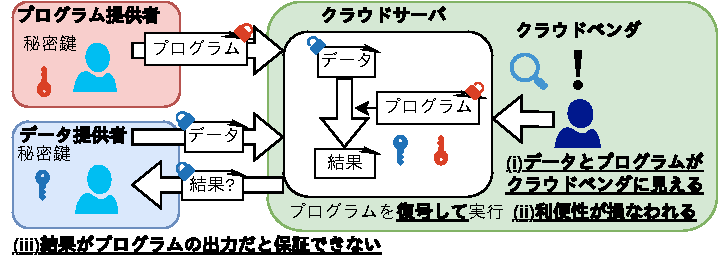
\includegraphics[width=0.8\linewidth]{figures/problem.drawio.pdf}
    \vspace*{-0.5cm}
    \caption{既存のクラウドコンピューティングの問題点}
    \label{fig:problem}
\end{figure}

\noindent[\textbf{課題・分野の状況}]
% 及びー
% 着想に至った経緯にまとめる
% 現状を書く
% ここ短くする
% 現状はいかにまとめる
\begin{enumerate}[label=(\roman*),leftmargin=0.5cm]
\setlength{\parskip}{0cm} % 段落間
\setlength{\itemsep}{0cm} % 項目間
% パラレルにする(利便性の維持を変更するか他を合わせる
    \item \underline{\textbf{データとプログラムがクラウドベンダに見える}}: 図1に示すように、クラウドコンピューティングではサーバ上でデータとプログラムは復号される。準同型暗号を用いれば暗号化したまま計算を行えるが、webサービスのようにプログラム提供者とデータ提供者が分かれる場合、計算量が鍵の本数の2乗に比例する[1]という問題がある。\label{prob:maliciousvender}
    \item  \underline{\textbf{利便性が損なわれる}}: 我々の過去の研究[4]では暗号化したままC言語を実行可能である。しかし、独自ISAを採用したためにコンパイラも独自であり、他の言語がサポートできていない。\label{prob:usability}
    \item  \underline{\textbf{実行結果がプログラムの出力だと保証できない}}: クラウドベンダはコストを抑えるため、プログラムを実行せず偽の結果を返す可能性がある。\amikake{\textbf{Verifiable Computation(VC)}}を用いれば結果がプログラムの実行結果であるかを検証できる。しかし、適用された準同型暗号が限られている[2]か、実装が存在しない[3]。\label{prob:verifiability}
\end{enumerate}

\noindent[\textbf{着想に至った経緯}]
% 自身の前の研究を欠陥を指摘する感じに

準同型暗号を知った時、「これが論理関数(NAND)を計算できるのであれば、暗号のまま計算処理をするCPUが作れるはずだ」と考えた。本研究はこの発想を骨子として現代的コンピュータの進化形として構想した。

%end 本研究の着想に至った経緯など ====================

% p01_background_01.tex
\KLEndSubject{F}



%#Split: 02_purpose_plan  
%#PieceName: p02_purpose_plan
% p02_purpose_plan_00.tex
\KLBeginSubjectWithHeaderCommands{02}{}{研究目的・内容等}{2}{F}{}{\DCPDFirstSubjectPageStyle}{\DCPDDefaultPageStyle}

\section{研究目的・内容等}
%    <<最大 2ページ>>

%s02_purpose_plan_dcpd
%begin 研究目的と研究計画short留意事項なし ====================
\noindent[\textcircled{1}\textbf{研究目的}]

本研究の理想は「クラウドベンダ」への信用を「クラウドコンピューティング」から取り除くことである。そのための一歩として本研究では、プログラム提供者とデータ提供者が異なる(1)線形計算量3パーティ拡張を(2)暗号上プログラム実行基盤として利便性を保ちながら行い、(3)計算結果の検証も可能にすることを目指す。図2にこれらを統合した本研究で提案するプロトコルを示す。

% (1)を真ん中に(3)を下に
% ロックと鍵を小さく
\begin{figure}[h]
    \centering
    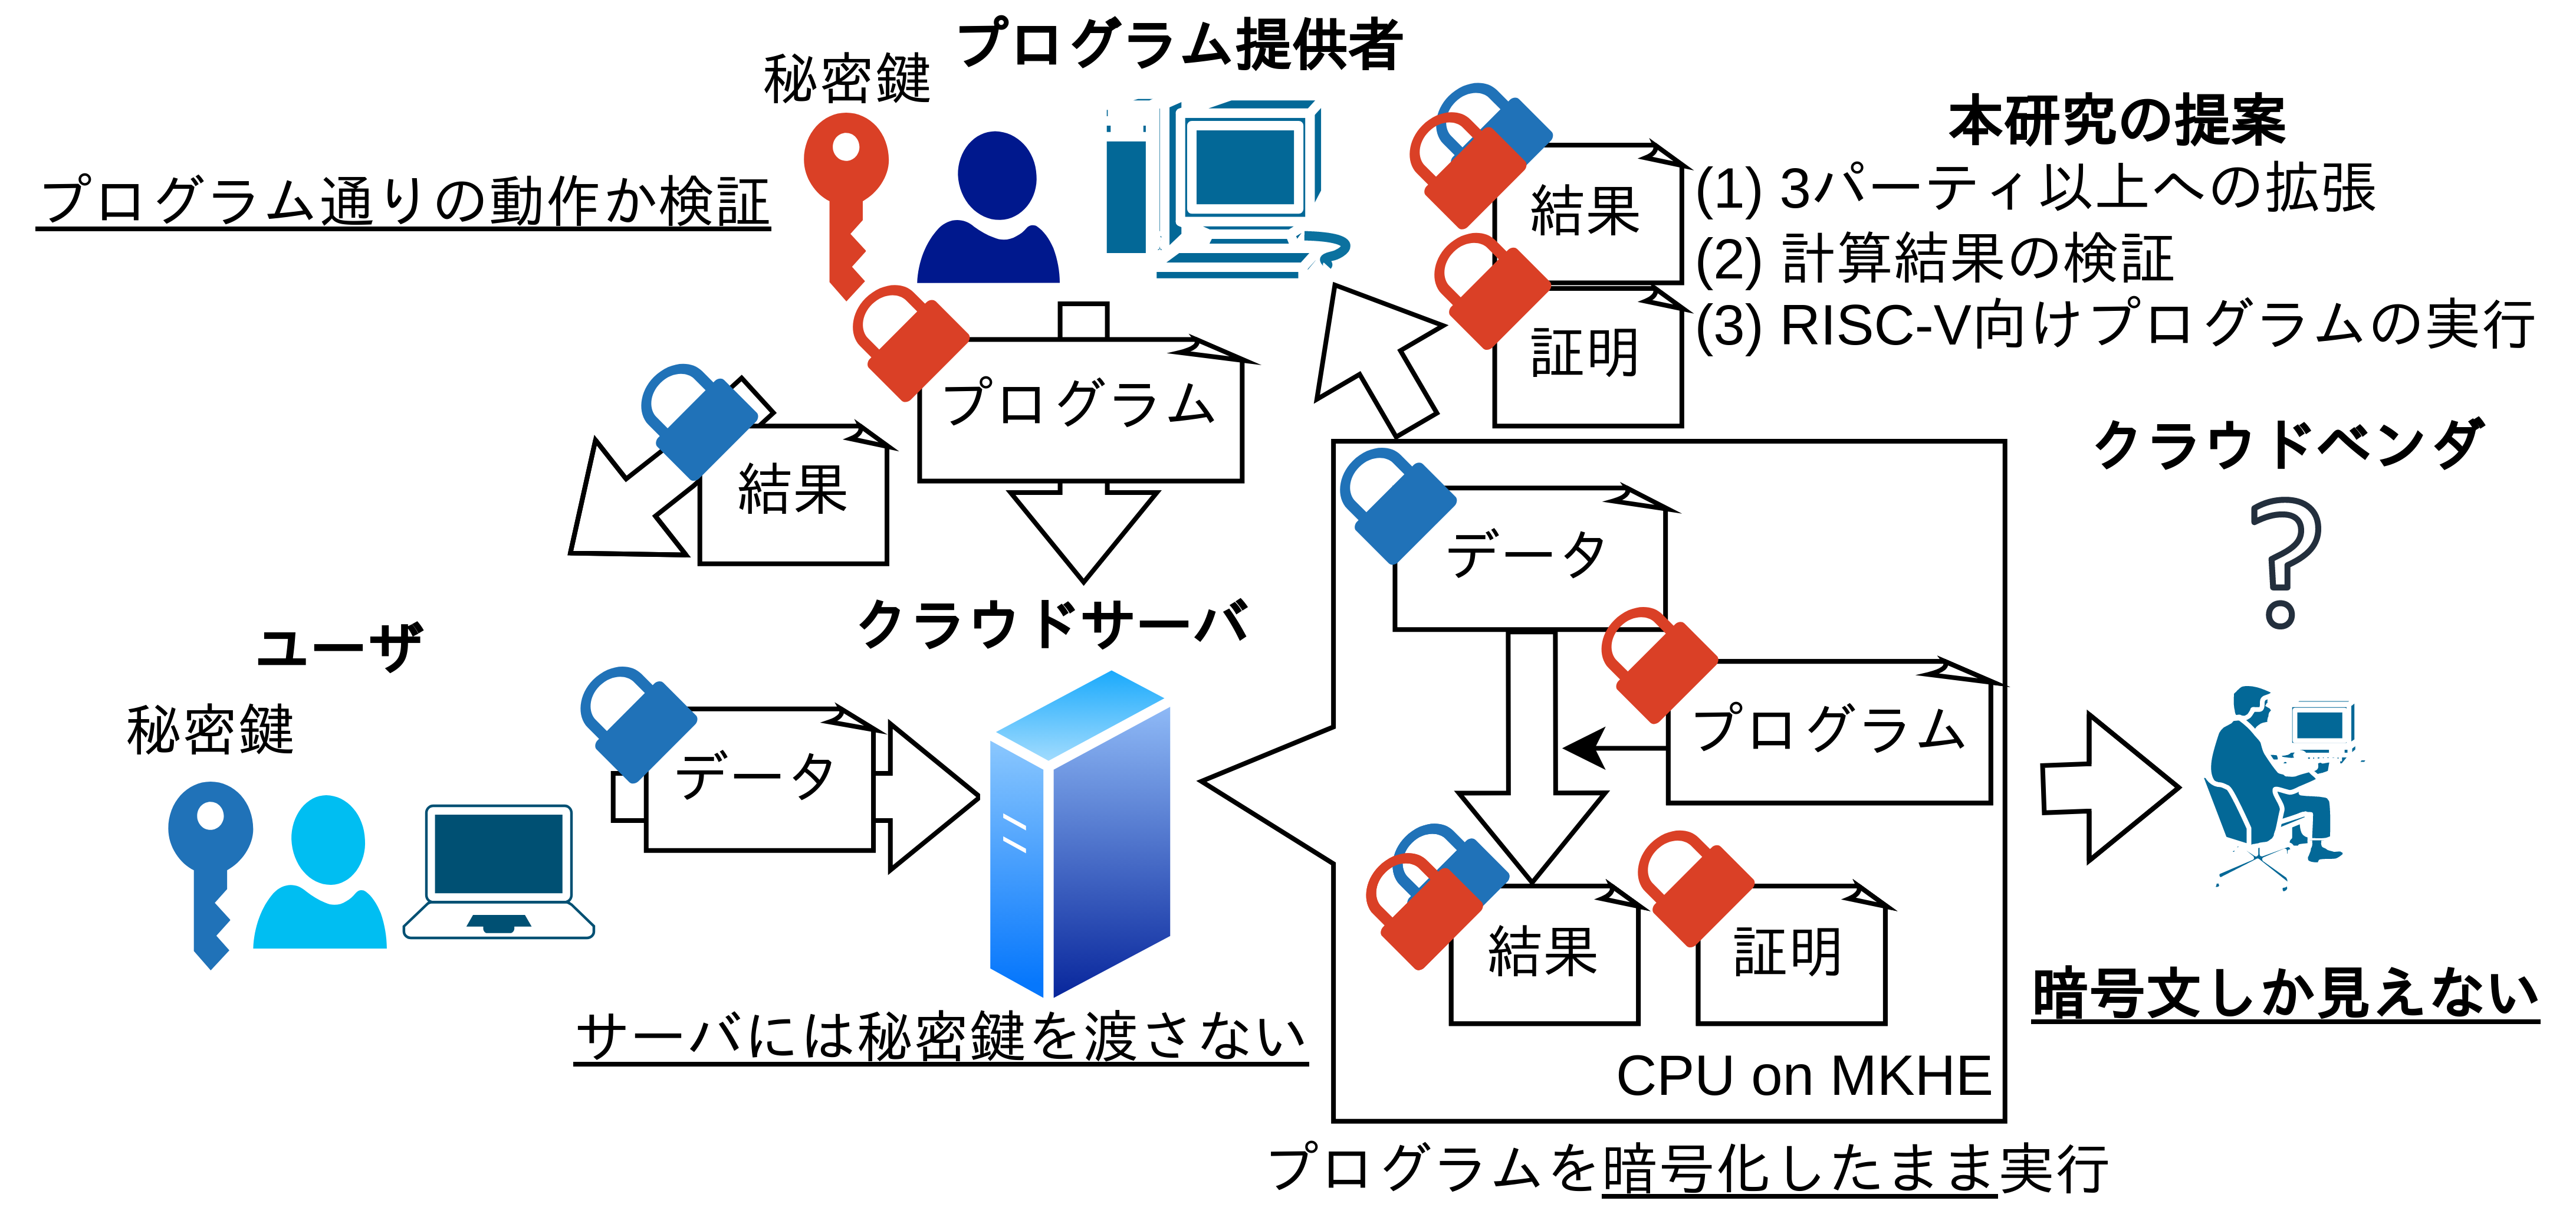
\includegraphics[width=0.8\linewidth]{figures/solution.drawio.png}
    \vspace*{-0.5cm}
    \caption{Caption}
    \label{fig:solution}
\end{figure}

\noindent [\textcircled{1}\textcircled{2}\textcircled{4}\textbf{研究内容・研究方法・どこまで明らかにするか・申請者が担当する部分}]

以下はすべて申請者が担当する。

\noindent(1) 線形計算量3パーティ拡張

MK-TFHE[1]はプログラム提供者とプログラム提供者が異なる3パーティ環境において、(i)データとプログラムがクラウドベンダに見えることを防げる。しかし、計算量が鍵の本数の2乗に比例する欠点がある。本項目では近年提案された他の準同型暗号向けの手法[5,6]をMK-TFHEに適用することにより論理回路に適した準同型暗号で計算量を鍵の本数に線形に比例させる方法を明らかにする。

\noindent(2) 暗号上プログラム実行基盤

 (1)により暗号化したまま計算することは可能である。しかし、計算を準同型暗号特有の表現に変換する必要があり、通常のプログラムをそのまま実行することはできない。(iii)利便性の維持のために、本項目ではRISC-V CPUの論理回路を暗号上で実行することで、通常のプログラムをそのまま実行可能にする方法を明らかにする。しかし、この方法はCPUの回路には準同型暗号特有の制約が生じる。そのため、使用可能な論理ゲート、(1)による影響、準同型暗号を実行するCPU・GPU・FPGAの特性などを考慮した最適なマイクロアーキテクチャも明らかにする

(3)	計算結果の検証

 (ii) 実行結果がプログラムの出力だと保証できないことは、準同型暗号にVCを統合することで解決できる。そのような手法には、(a)準同型暗号の実行自体を検証する物[2]と、(b)準同型暗号の上の計算を検証する物[3]の2種類がある。本項目では(1)と(2)の成果と統合する上で(a),(b)のどちらがセキュリティ的・性能的に優れているかを明らかにし、その実装を与える。

\noindent[\textcircled{\scriptsize 2}\textbf{研究計画}]

\noindent(申請時点から採用までの準備)
% MICROの内容は計画にする

申請時点で知る限り最速な準同型暗号のFPGA実装に成功しており、この成果は国際会議に投稿予定である。これに加え、(2)暗号上プログラム実行基盤の実装に向け、CPU・GPU向け準同型暗号ライブラリの最新の知見の統合による高速化と、準同型暗号の並列実行のためのジョブディスパッチャの複数マシンへの拡張を行う。この成果は論理回路の準同型暗号上での高速な実行基盤として国際会議に投稿予定である。

\noindent(1年目: (1)線形計算量3パーティ拡張)

採用前から改善する暗号ライブラリにマルチパーティ拡張の知見[5,6]を統合し、理論的・実装的に高速化する。この成果はマルチパーティ向け準同型暗号の理論的・実装的改善として国際会議に投稿する。

\noindent(2年目: (2)暗号上プログラム実行基盤の実装)

採用前と1年目の成果に加え、準同型暗号特有の制約を考慮した最適なCPUのアーキテクチャを開発することで、既存プログラムの暗号上での高速な実行を実現し、国際会議で発表する。
 
\noindent(3年目:(3)計算結果の検証)

ここまでの成果にVCの知見を統合し、準同型暗号上でのプログラム実行を検証可能にする。この成果は検証可能かつ3パーティでの既存プログラムの暗号上実行手法として国際会議で発表する。

\begin{figure}[h]
    \centering
    
\includegraphics[width=\linewidth]{figures/schedule.drawio.png}
    \vspace*{-1cm}
    \caption{schedule}
    \label{fig:schedule}
\end{figure}

\noindent[\textcircled{3} \textbf{特色・独創的な点}]

 本研究は準同型暗号上でRISC-V CPUの論理回路を評価することで、既存のプログラムを暗号化したまま実行可能としつつ、3パーティかつ計算結果が検証可能という高いセキュリティを達成することが独創的な点である。特色ある点は本研究では準同型暗号ライブラリ、計算の検証、準同型暗号並列実行のためのジョブディスパッチャ、準同型暗号上で実行するRISC-V CPUをプラットフォームとして実装する点である。

\noindent[\textcircled{3}先行研究との比較]

\noindent(1)	本研究ではCPUの論理回路を実行するため、それに適した準同型暗号を用いる。3パーティに対応したそのような既存の暗号がMK-TFHE[1]である。しかし、計算量が鍵の本数の2乗に比例する欠点がある。本研究では論理回路実行に適した計算量が鍵の本数に線形に比例する準同型暗号を開発する。

\noindent(2)	我々の過去の研究[4]では2パーティに限られ、計算の検証は行えていなかった。また、独自ISAのため、C言語のみのサポートにとどまっていた。本研究ではRISC-V ISAを採用することでより多くの言語をサポートする。また。過去の研究よりも多くの側面を考慮に入れた最適なマイクロアーキテクチャを明らかにする最初の研究である。

\noindent(3)	準同型暗号と計算の検証を同時に行う研究は、MK-TFHEに適応できていない[1]か、実装が存在しない[2]。本研究は既存プログラムの暗号上実行に適した検証法を検討し、実装を与える最初の研究である。

\noindent[\textcircled{3}本研究が完成したとき予想されるインパクト及び将来の見通し]

 本研究完成の暁には、クラウドベンダへの信用が取り除かれることにより、社会活動における特定の大企業への依存が低減されると考えている。将来の見通しとしてはクラウドコンピューティングから信用を取り除くことは、個人情報を収集して解析するニーズに対し、暗号学的にデータの安全性を担保した計算基盤を提供するための一歩となると考えている。

\noindent[参考文献] [5] T. Kim, et.al, “Asymptotically Faster Multi-Key Homomorphic Encryption from Homomorphic Gadget Decomposition.” IACR Cryptology ePrint Archive, 2022. [6] X. Dai, et.al. “Key lifting : Multi-key Fully Homomorphic Encryption in plain model.” IACR Cryptology ePrint Archive, 2022.


%end 研究目的と研究計画short留意事項なし ====================
% p02_purpose_plan_01.tex
\KLEndSubject{F}



%#Split: 03_rights  
%#PieceName: p03_rights
% p03_rights_00.tex
\KLBeginSubjectWithHeaderCommands{03}{3}{人権の保護及び法令等の遵守への対応}{1}{F}{}{\DCPDFirstSubjectPageStyle}{\DCPDDefaultPageStyle}

\section{人権の保護及び法令等の遵守への対応}
%    <<最大 1ページ>>

% s09_rights
%begin 人権の保護及び法令等の遵守への対応 ====================
	象の卵のES細胞の培養、象のクローンの生成などは行わない。

	\LaTeX の便利な機能については、\texttt{egg\_***.tex} や\texttt{sample\_pdf/egg\_***.pdf}をご覧ください。
%end 人権の保護及び法令等の遵守への対応 ====================

% p03_rights_01.tex
\KLEndSubject{F}



%#Split: 04_abilities  
%#PieceName: p04_abilities
% p04_abilities_00.tex
\KLBeginSubjectWithHeaderCommands{04}{4}{研究遂行力の自己分析}{2}{F}{}{\DCPDFirstSubjectPageStyle}{\DCPDDefaultPageStyle}

\section{研究遂行力の自己分析}
%    <<最大 2ページ>>

% s14_abilities
%begin 自己分析 ====================
% \DCPDInstructionsA\\% <-- 留意事項:これは消すか、コメントアウトしてください。
\noindent\textbf{(1) 研究に関する自身の強み}
% \DCPDInstructionsB% <-- 留意事項:これは消すか、コメントアウトしてください。

\noindent・\textbf{知識の幅・深さ、技量}

本申請を実施するうえで応募者の最大の強みと言えるのは、使用するソフトウェアの多くを自分で開発・保守を行ってきていることである。
中核となる準同型暗号ライブラリはCPU・GPU・FPGA用の3種類を開発しており、それらを用い論理回路を評価する実行エンジン、暗号上で動かすプロセッサまで研究に必要な幅広いソフトウェアをカバーしている~[\ref{code:vsp}]。
特に準同型暗号ライブラリの実装については情報処理推進機構のセキュリティキャンプにて講師として招聘された他~[\ref{achieve:seccamp}]、企業でのパートタイムジョブとしても行いその成果を査読付き国際ワークショップで発表する~[\ref{paper:wahc}]など、高い水準にある。
学部2,3年の時にはNHK学生ロボコンにて優勝~[\ref{achieve:nhk}]、専門分野を超えたハード・ソフトを問わない技量を養った。

\noindent・\textbf{研究における主体性}

申請者は高校生で最初の論文~[\ref{paper:rfid}]を出版しており、このときから研究との向き合い方を学んできた。
特に本申請の研究計画の核となる準同型暗号に関するテーマは、申請者は学部3年生の時点から継続して3年以上取り組んできた。
学部3年生のときに発案したテーマは、情報処理推進機構の未踏事業に採択、スーパクリエータとして認定され~[\ref{achieve:mitou}]、京都大学総長賞も受賞~[\ref{achieve:vsp}]、成果は査読付き国際学会に採択~[\ref{paper:usenix}]された。
研究室の継続的指導のない状態で研究を行えたことは主体性の証左であると考える。

\noindent・\textbf{発想力・問題解決能力}

学部2回生で準同型暗号を知り、もし準同型暗号がNANDを計算できるのであれば、暗号上でプロセッサが評価できると考えた。
最初に発案した準同型暗号のテーマ~[\ref{paper:usenix}]から始まり、本申請に至るまで、このアイデアに基づいており、プログラムとデータの両方を暗号によって保護するセキュリティと通常のCPUのような使い勝手という利便性をより広い条件で達成するべく進めている。
暗号上でのメモリ評価の高速化~[\ref{paper:usenix}]や、より複雑な論理ゲートの実現~[\ref{paper:wahc}]など、暗号上でのCPUの評価における問題をこれまで解決してきている。
また、準同型暗号の応用という面では、プロセッサの評価以外にもオートマトン~[\ref{paper:cav}]やBinalized Neural Network~[\ref{achieve:bnn}]なども試みており、分野をまたいだアイデアの実現に取り組んできた。
長期的な研究につながるアイデアと分野をまたいだ応用のアイデアに取り組み、その実現のために様々な問題を解決してきたことは申請者の高い発想力と問題解決能力の証と考える。

\noindent・\textbf{コミュニケーション力}
% 学外の人との関わり

未踏に採択されたチームは異なる背景を持った現在の所属研究室も異なる人間であり、技術的意見の相違から衝突することもままあるが、申請時点まで共同での研究を維持できている。
また、セキュリティキャンプでは毎年異なる学生に少人数でのゼミを行ってきた。
これらは申請者のコミュニケーション能力の傍証と考える。

\noindent・\textbf{プレゼンテーション力}

申請者は招待講演を含む国内外の会議で発表実績があり~[\ref{achieve:wcis}]、対外的な発表能力も身につけている。

\noindent\textbf{成果-レター誌・査読あり}
\begin{enumerate}[leftmargin=0.5cm]
    \setlength{\parskip}{0cm} % 段落間
    \setlength{\itemsep}{0cm} % 項目間
	\paper{An RFID tag identification protocol via Boolean compressed sensing,}{Kotaro Matsuoka \etal}{IEICE Communications Express, Volume 5, Issue 5}{}{118-123}{2016}\label{paper:rfid}
\end{enumerate}

\noindent\textbf{成果-国際学会またはワークショップでの発表・口頭・査読あり}
\begin{enumerate}[leftmargin=0.5cm]
    \setcounter{enumi}{1}
    \setlength{\parskip}{0cm} % 段落間
    \setlength{\itemsep}{0cm} % 項目間
    \paper{Virtual Secure Platform: A {Five-Stage} Pipeline Processor over {TFHE}}{Kotaro Matsuoka, \etal}{30th USENIX Security Symposium (USENIX Security 21)}{}{4007--4024}{Online, 2021年月}\label{paper:usenix}
    \paper{Oblivious Online Monitoring for Safety LTL Specification via Fully Homomorphic Encryption}{Ryotaro Banno, Kotaro Matsuoka \etal}{Computer Aided Verification}{}{}{2022年8月}\label{paper:cav}
    \paper{Towards Better Standard Cell Library: Optimizing Compound Logic Gates for TFHE
Association for Computing Machinery}{Kotaro Matsuoka, \etal}{In Proceedings of the
9th on Workshop on Encrypted Computing \& Applied Homomorphic Cryptography (WAHC '21), Association for Computing Machinery (ACM)}{}{pp.63–68}{Online, 2021年11月}\label{paper:wahc}
\end{enumerate}

\noindent\textbf{成果-国内学会またはシンポジウムでの発表・口頭・査読なし}
\begin{enumerate}[leftmargin=0.5cm]
    \setcounter{enumi}{4}
    \setlength{\parskip}{0cm} % 段落間
    \setlength{\itemsep}{0cm} % 項目間
     \item  完全準同型暗号における BNN を用いた高速な秘匿推論手法の実装と評価. 情報処理学会全国大会 橋詰陽太,古川修平,松本直樹,伴野良太郎,松岡航太郎,佐藤高史. 2022 年 3 月. オンライン.\label{achieve:bnn}
	\item  Virtual Secure Platform: A Five-Stage Pipeline Processor over TFHE (from Usenix Security 2021). 暗号と情報セキュリティワークショップ(WCIS 2021)招待講演, オンライン, 2021年9月 \label{achieve:wcis}
	\item  Virtual Secure Platform: A Five-Stage Pipeline Processor over TFHE. FIT2022 招待講演, オンライン, 2022年9月\label{achieve:fit}
\end{enumerate}


\noindent\textbf{成果-受賞}
\begin{enumerate}[leftmargin=0.5cm]
    \setcounter{enumi}{7}
    \setlength{\parskip}{0cm} % 段落間
    \setlength{\itemsep}{0cm} % 項目間
	\paper{2019 年度 IPA 未踏 IT 人材発掘・育成事業 スーパクリエータ「準同型暗号によるバーチャルセキュアプラットフォームの開発」}{松岡 航太郎}{\url{https://www.ipa.go.jp/files/000082597.pdf}}{}{}{2019}\label{achieve:mitou}
	\paper{令和元年度 京都大学総長賞 (NHK学生ロボコン2019~ABUアジア・太平洋ロボコン代表選考会~ 優勝、チェコ杯・NOK賞受賞、 ABUアジア・太平洋ロボコン選考会ベスト8、ナガセ賞、ベストデザイン賞受賞)}{京大機械研究会}{\url{https://www.kyoto-u.ac.jp/sites/default/files/embed/jaeducation-campusRecognitionpresidentsdocuments2019zyusyousyalist.pdf}}{}{}{2020}\label{achieve:nhk}
	\paper{令和 2 年度 京都大学総長賞}{松岡 航太郎 \etal}{\url{https://www.kyoto-u.ac.jp/sites/default/files/inline-files/r2-sochosho-jyusho-168da1573b39e3ca3fa2c6c362417307.pdf}}{}{}{2021}\label{achieve:vsp}
	\item CSS2021 優秀論文賞 \url{https://www.iwsec.org/css/2021/award.html} \label{achieve:css}
\end{enumerate}


\noindent\textbf{成果-公開ソフトウェア}
\begin{enumerate}[leftmargin=0.5cm]
    \setcounter{enumi}{11}
    \setlength{\parskip}{0cm} % 段落間
    \setlength{\itemsep}{0cm} % 項目間
	\item Virtual Secure Platform, \url{https://github.com/virtualsecureplatform}\label{code:vsp}
\end{enumerate}

\noindent\textbf{成果-その他活動}

\begin{enumerate}[leftmargin=0.5cm]
    \setcounter{enumi}{12}
	\item セキュリティキャンプ 全国大会 2020-2022 L-2 暗号のまま計算しようゼミ 講師 及び 2022 Lトラックプロデューサ, \url{https://www.ipa.go.jp/jinzai/camp/2022/zenkoku2022_program_profile.html}\label{achieve:seccamp}
\end{enumerate}

\vspace{5mm}
\noindent\textbf{(2) 今後研究者として更なる発展のため必要と考えている要素}



\noindent\textbf{要素1: 研究成果を論文としてまとめる能力}

これまでの論文執筆では、指導教員等からの指導が不可欠であったと感じている。
より高い執筆能力を獲得することは論文の投稿にかかるコストを下げより多くの研究に取り組むことを可能にすると同時に、論文化を意識した研究計画を立てる助けになるものである。
よって、成果を論文としてまとめる能力は研究者としてさらなる発展のため必要と考えている。

\noindent\textbf{要素2:暗号学の基礎的知識}

ここでいう暗号学の基礎的知識というのは、2つの意味合いを持つ。
一つにはどういうものならば安全であるか、という安全性の前提に関する知識である。
準同型暗号は安全性よりもその機能に重点が置かれやすく、機能の改善のために既存の安全生証明とは異なる仮定を課すことがある。
そのような仮定が安全であるかを、拡張の提案と同時に議論できる能力の獲得はより広範な研究テーマに取り組むことを可能にするものと考えている。
もう一つの意味合いは、ブロックチェーンなどの準同型暗号以外の暗号技術への一定程度の理解である。
本申請でVerfifiable Computationの統合を目指すように、準同型暗号単体では達成できないセキュリティが存在する。
よって、どのような技術を組み合わせればより高い次元のセキュリティが達成できるかの指針を得るのに十分な程度の知識を持つことはより広範な研究アイデアの発案につながるものと考える。

%end 自己分析 ====================

% p04_abilities_01.tex
\KLEndSubject{F}



%#Split: 05_my_ambitions  
%#PieceName: p05_my_ambitions
% p05_my_ambitions_00.tex
\KLBeginSubjectWithHeaderCommands{05}{5}{目指す研究者像等}{1}{F}{}{\DCPDFirstSubjectPageStyle}{\DCPDDefaultPageStyle}

\section{目指す研究者像等}
%    <<最大 1ページ>>

% s17_my_ambitions
\noindent
\textbf{(1)目指す研究者像 {\footnotesize ※目指す研究者像に向けて身に付けるべき資質も含め記入してください。}}

%begin 目指す研究者像 ====================
% 資質について書く
% 1.と海外にする

\noindent\textbf{\textcircle{1}高校時代の自分の助けになるような情報発信}

私が人生で初めて読んだ論文は後保範先生の博士論文であり、この論文で学んだ高速乗算法が準同型暗号の高速化に生きている。
この経験から、オープンアクセスの論文は誰もが入手できる専門的かつ信頼性の高い情報源であり、高校生が大学院レベルの知識を得ることも可能にする公益性の高いものだと信じている。
勿論、前提知識なしに論文を読み解くことは難しく、書籍やブログなど、それ以外の補助的な情報発信も必要である。
この自身の経験を次の世代も得られるよう、最先端の知見をオープンに発信していくことが目指すべき姿であると考えている。
具体的には、自らの論文はすべてオープンアクセスまたはプレプリントを公開し、セキュリティキャンプのような教育的な情報発信の機会には積極的に参加、SNSやブログなどでも補助的な情報を発信。
また、論文はその時の最新の知識を提供するものであるが、自分の知識を体系化し後世に伝える書籍を執筆することが人生の目標の一つである。

\noindent\textbf{\textcircle{2}幅広い専門性の獲得}

私の座右の銘の一つは「アイデアは自分の子供」である。
アイデアを実現できるかできないかというのは発案した者の双肩にかかるものであり、最終的に諦めるのだとしても最大限の努力を払ってからにすべきであると考える。
この座右の銘を研究者としてのあり方に適用するならば、自分の能力の及ぶ限り研究アイデアの実施を試みるということであり、より具体的には実施するための幅広い専門性を獲得することが目指すべき研究者像であると考える。
幅広い専門性が必要と考えるのは、研究アイデアは自分の専門分野にとどまるものとは限らないと認識しているためである。
実際、私が最初の準同型暗号に関連する研究テーマを思いついたのは、準同型暗号という名前と「暗号のまま計算できる」という性質だけを知ったときで、準同型暗号に関する知識はまったくなかった。
研究アイデアの実現に自分の専門分野の外の知識が必要なとき、その学習コストを支払うことをためらわないのが目指すべき研究者像であると考える。

\noindent\textbf{\textcircle{3}オープンソース実装による再現性の確保}

良い研究の必須要件の一つは、再現性が十分に確保されていることだと考えている。
実験や評価の結果が再現できなければ、ハードウェアの進歩などで環境が変わった場合に公正な比較ができない。
そのため、研究で作成したソフトウェア・ハードウェアはオープンソースにし後世の研究で自由に使えるようにすることが望ましい研究者像だと考えている。

% \noindent\textbf{2.2 単独で研究を続行できる幅広い専門性の獲得}

% 専門外の分野に踏み出す場合などは、他者の助力を請う事は多くの場合望ましいことである。
% しかし。研究の実施を他者に依存しきると、何らかの理由で助力を得ることが難しくなったときに研究を継続できなくなる。
% よって、規模の縮小などは致し方ないが、そのような場合も研究を単独で遂行できるだけの幅広い専門性を研究の過程で獲得できることが目指す研究者像であると考える。
 %end 目指す研究者像 ====================

\vspace{5mm}
\noindent
\textbf{(2)上記の「目指す研究者像」に向けて、特別研究員の採用期間中に行う研究活動の位置づけ}

\noindent\textbf{\textcircle{1} 高校時代の自分の助けになるような情報発信}

採用中に執筆する論文はすべてオープンアクセスにするか、プレプリントを公開する。
また、研究内容をTwitterで発信したり、Qiitaで基礎的な知識の解説を研究活動の一環として行いたいと考えている。

\noindent\textbf{\textcircle{2} 幅広い専門性の獲得}

本申請の研究計画の範囲はVerifiable Computationやプロセッサ設計など幅のあるものではあるが、ある程度基礎的な知識を得ている範囲で計画している。
これらに加え、エフォートの一部をブロックチェーンや疑似乱数などの暗号学の中の他分野や、機械学習などの応用としての他分野を学習することに当てたいと考えている。

\noindent\textbf{\textcircle{3} オープンソース実装による再現性の確保}

採用中に開発するハードウェア・ソフトウェアはApache系またはGPL系のライセンスの元でオープンソースとして公開する。
実行環境もパブリッククラウドを利用するなど可能な範囲で再現性に配慮する。

%begin 研究活動の位置づけ ====================
% 実際に身につけるための活動を書く
% 論文のオープン化
% 他研究室との共同研究



%end 研究活動の位置づけ ====================

% p05_my_ambitions_01.tex
\KLEndSubject{F}



%#Split: 99_tail
% hook9 : right before \end{document} ============
 % pieces
\end{document}

